\vspace*{1.5mm}
\block{\strut 1. Scientific context, motivation, and approach}{

        \vspace{0.3cm}

        \textbf{High-resolution transmission electron microscopy (HRTEM)} provides direct access to the structure and morphology of nanoalloys, but image interpretation remains \textbf{challenging and expert-dependent}.
        \textbf{Deep learning} can accelerate this analysis --- provided a \textbf{large, representative dataset} is available.
        We generate such a dataset from \textbf{molecular dynamics} snapshots and synthetic HRTEM images produced via the \textbf{multislice} method.

        \vspace{0.6cm}

        \textbf{The \textcolor{colorAg}{Ag}--\textcolor{colorCo}{Co} system:} an immiscible nanoalloy:\\
        \textcolor{colorAg}{\textbf{Ag}} $\rightarrow$ \textbf{surface} (lower surface energy, larger atoms), \\
        \textcolor{colorCo}{\textbf{Co}} $\rightarrow$ \textbf{core}.\\
        Metastable conformations possible depending on synthesis conditions:

        \vspace{0.5cm}

        \begin{center}
            \begin{tikzpicture}[x=\linewidth, y=1cm]
                \node[inner sep=0] (img1) at (0.17,4.5) {
                    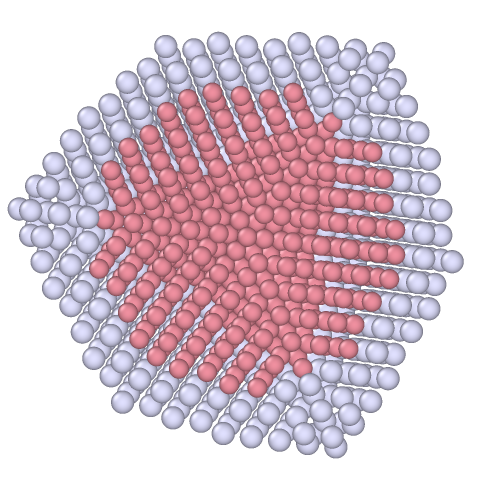
\includegraphics[height=8cm]{Figure/cs.png}
                };
                \node[font=\small\bfseries] at (0.17,0.0) {Core--shell};

                \node[inner sep=0] (img2) at (0.50,4.5) {
                    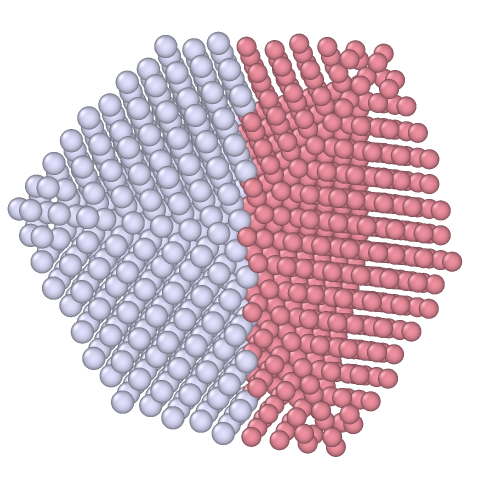
\includegraphics[height=8cm]{Figure/janus.png}
                };
                \node[font=\small\bfseries] at (0.50,0.0) {Janus};

                \node[inner sep=0] (img3) at (0.83,4.5) {
                    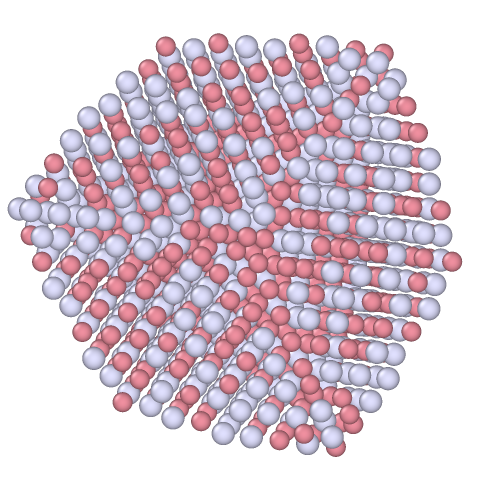
\includegraphics[height=8cm]{Figure/random.png}
                };
                \node[font=\small\bfseries] at (0.83,0.0) {Mixed};
            \end{tikzpicture}
        \end{center}

        \vspace{0.6cm}

        \textbf{\underline{Workflow overview}}

        \vspace{0.5cm}

        \begin{center}
            \begin{tikzpicture}[x=\linewidth,y=9cm]
                \fill[approachOne] (0.00,0.04) -- (0.24,0.04) -- (0.32,0.50) -- (0.24,0.96) -- (0.00,0.96) -- cycle;
                \fill[approachTwo] (0.29,0.04) -- (0.55,0.04) -- (0.63,0.50) -- (0.55,0.96) -- (0.29,0.96) -- (0.37,0.50) -- cycle;
                \fill[approachThree] (0.60,0.04) -- (0.88,0.04) -- (0.96,0.50) -- (0.88,0.96) -- (0.60,0.96) -- (0.68,0.50) -- cycle;

                \node[align=left, text width=0.17\linewidth, font=\bfseries] at (0.13,0.52) {Generate\\nanoalloy\\configurations};
                \node[align=left, text width=0.18\linewidth, font=\bfseries] at (0.46,0.52) {Simulate HRTEM\\images and\\extract structural\\parameters};
                \node[align=left, text width=0.18\linewidth, font=\bfseries] at (0.79,0.52) {Train and apply\\deep-learning\\models};
            \end{tikzpicture}
        \end{center}

}
